\NeedsTeXFormat{LaTeX2e}
\documentclass[a4paper,12pt,
headsepline,           % Linie zw. Kopfzeile und Text
oneside,               % einseitig
pointlessnumbers,      % keine Punkte nach den letzten Ziffern in Überschriften
bibtotoc,              % LV im IV
%DIV=15,               % Satzspiegel auf 15er Raster, schmalere Ränder   
BCOR15mm               % Bindekorrektur
%,draft
]{scrbook}
\KOMAoptions{DIV=last} % Neuberechnung Satzspiegel nach Laden von Paket helvet

\pagestyle{headings}
\usepackage{blindtext}

% für Texte in deutscher Sprache
\usepackage[english]{babel}
\usepackage[utf8]{inputenc}
\usepackage[T1]{fontenc}

% Helvetica als Standard-Dokumentschrift
\usepackage[scaled]{helvet}
\renewcommand{\familydefault}{\sfdefault} 

\usepackage{graphicx}

% Literaturverzeichnis mit BibLaTeX
\usepackage[babel,german=quotes]{csquotes}
\usepackage[backend=bibtex8]{biblatex}
\bibliography{bibliography}

% Alternative mit Paket-Option backend=biber und \addbibresource
% \usepackage[backend=biber]{biblatex}
% \addbibresource{bibliography.bib}

% Für Tabellen mit fester Gesamtbreite und variabler Spaltenbreite
\usepackage{tabularx} 

% Besondere Schriftauszeichnungen
\usepackage{url}              % \url{http://...} in Schreibmaschinenschrift
\usepackage{color}            % zum Setzen farbigen Textes

\usepackage{amssymb, amsmath} % Pakete für Mathe-Umgebungen und -Symbole

\usepackage{setspace}         % Paket für div. Abstände, z.B. ZA
%\onehalfspacing              % nur dann, wenn gefordert; ist sehr groß!!
\setlength{\parindent}{0pt}   % kein linker Einzug der ersten Absatzzeile
\setlength{\parskip}{1.4ex plus 0.35ex minus 0.3ex} % Absatzabstand, leicht variabel

% Tiefe, bis zu der Überschriften in das Inhaltsverzeichnis kommen
\setcounter{tocdepth}{3}      % ist Standard

% Beispiele für Quellcode
\usepackage{listings}
\lstset{language=Java,
  showstringspaces=false,
  frame=single,
  numbers=left,
  basicstyle=\ttfamily,
  numberstyle=\tiny}

% custom
\usepackage{minted}
\usepackage{svg}
\usepackage{longtable}

% hier Namen etc. einsetzen
\newcommand{\fullname}{Matthias Klenz}
\newcommand{\email}{matthias.klenz@uni-ulm.de}
\newcommand{\titel}{Development of a recommender system for process evaluation/modeling}
\newcommand{\jahr}{2023}
\newcommand{\matnr}{123456}
\newcommand{\gutachterA}{Prof.\,Dr.\,Streng Geheim}
\newcommand{\gutachterB}{Prof.\,Dr.\,Un Leserlich}
\newcommand{\betreuer}{Michael Winter}

% hier die Fakultät auswählen
%\newcommand{\fakultaet}{---  Im Quellcode anpassen nicht vergessen! ---}
\newcommand{\fakultaet}{Ingenieurwissenschaften, Informatik und\\Psychologie}
%\newcommand{\fakultaet}{Mathematik und\\Wirtschafts-\\wissenschaften}
%\newcommand{\fakultaet}{Medizin}
%\newcommand{\fakultaet}{Naturwissenschaften}

% hier das Institut einsetzen
\newcommand{\institut}{Institut für Datenbanken und Informationssysteme (DBIS)}

% Informationen, die LaTeX in die PDF-Datei schreibt
\pdfinfo{
  /Author (\fullname)
  /Title (\titel)
  /Producer     (pdfeTex 3.14159-1.30.6-2.2)
  /Keywords ()
}

\usepackage{hyperref}
\hypersetup{
pdftitle=\titel,
pdfauthor=\fullname,
pdfsubject={Diplomarbeit},
pdfproducer={pdfeTex 3.14159-1.30.6-2.2},
colorlinks=false,
pdfborder=0 0 0	% keine Box um die Links!
}

% Trennungsregeln
\hyphenation{Sil-ben-trenn-ung}

\begin{document}
\frontmatter

% Titelseite
\thispagestyle{empty}
\begin{addmargin*}[4mm]{-10mm}

\hfill

\includegraphics[height=1.8cm]{images/logo_uulm_sw.png}\\[1em]

{\footnotesize
%{\bfseries Universität Ulm} \textbar ~89069 Ulm \textbar ~Germany
\hspace*{115mm}\parbox[t]{35mm}{\bfseries Faculty for\\
\fakultaet\\
% TODO hier Institut anpassen
\mdseries \institut}\\[2cm]

\parbox{140mm}{\bfseries \LARGE \titel}\\[2.5em]
{\footnotesize Thesis at the university Ulm}\\[3em]

{\footnotesize \bfseries Submitted by:}\\
{\footnotesize \fullname\\ \email}\\ \matnr\\[2em]
{\footnotesize \bfseries Reviewers:}\\                     
{\footnotesize \gutachterA\\ \gutachterB}\\[2em]
{\footnotesize \bfseries Supervisor:}\\ 
{\footnotesize \betreuer}\\\\
{\footnotesize \jahr}
}
\end{addmargin*}


% Impressum
\clearpage
\thispagestyle{empty}
{ \small
  \flushleft
  Version \today \\\vfill
  \copyright~\jahr~\fullname\\[0.5em]
% Wenn Sie Ihre Arbeit unter einer freien Lizenz bereitstellen möchten, können Sie die nächste Zeile in Ihren Code aufnehmen. Bitte beachten Sie, dass Sie hierfür an allen Inhalten, inklusive enthaltener Abbildungen, die notwendigen Rechte benötigen! Beim Veröffentlichungsexemplar Ihrer Dissertation achten Sie bitte darauf, dass der Lizenztext nicht den Angaben in den Metadaten der genutzten Publikationsplattform widerspricht. Nähere Information zu den Creative Commons Lizenzen erhalten Sie hier: https://creativecommons.org/licenses/
This work is licensed under the Creative Commons Attribution 4.0 International (CC BY 4.0) License. To view a copy of this license, visit \href{https://creativecommons.org/licenses/by/4.0/}{https://creativecommons.org/licenses/by/4.0/} or send a letter to Creative Commons, 543 Howard Street, 5th Floor, San Francisco, California, 94105, USA. \\
  Satz: PDF-\LaTeXe
}

% ab hier Zeilenabstand etwas größer 
\setstretch{1.2}

\tableofcontents

\mainmatter
%\chapter{Introduction}

Diese kleine Einleitung soll dem Nutzer helfen selbst die eigene Arbeit mit \LaTeX{} zu schreiben. Sie enth"alt Beispiele zu den wichtigsten Themen .

\blindtext

\section{Dokumentlgiederung}

Für diese Arbeit verwendet man folgende LaTeX-Kommados zur Strukturierung:

\begin{verbatim}
\chapter{Einleitung}
\section{Dokumentgliederung}
\subsection{}
\subsubsection{}
\end{verbatim}

Allerdings sollte man sich überlegen, ob man wirklich bis zur Stufe \verb|subsubsection| "Uberschriften benötigt.

\section{Illustrationen}

\blindtext

\blindtext

\subsection{Bilder und Abbildungen}

Auch in einer wissenschaftlichen Arbeit können Bilder und Abbildungen zur Veranschaulichung und zur Illustration sachlicher Inhalte integriert und einfügt werden. Für Fotografien und Bilder unterstützt PDF-\LaTeX{} direkt \verb|jpg| und \verb|png|. Ansonsten empfiehlt es sich, Vektorgrafiken zu verwenden und diese als \verb|pdf| zu speichern. Sollte ein Bild einmal von zu viel weißem Raum umgeben sein, kann man mit dem Werkzeug \verb|pdfcrop| das Bild automatisch zuschneiden.

\begin{figure}[ht]
\centering
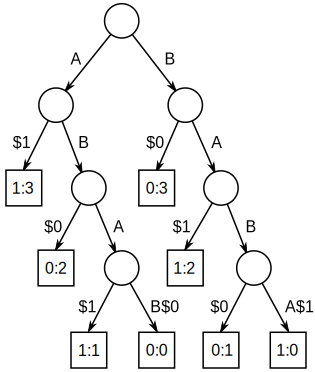
\includegraphics[width=.4\textwidth]{images/Suffix_tree_ABAB_BABA}
\caption{\label{fig:bild1}Beschreibung/Beschriftung des Bilds}
\end{figure}

Mit Hilfe eines Labels \verb|\label{fig:bild1}| kann man sich dann im fortlaufenden Text mittels eines Querverweises auf diese Grafik beziehen: \verb|\ref{fig:bild1}|. An der Stelle des ref-Kommandos platziert LaTeX die Nummer der Abbildung: \glq siehe Abbildung \ref{fig:bild1}\grq.


\subsection{Tabellen}
\label{sec:tabellen}

Seite \pageref{tab:beispieltabelle}, Abschnitt \ref{sec:tabellen}, enthält Beispieltabelle \ref{tab:beispieltabelle}. In vielen \LaTeX{}-Büchern finden sich gute Anleitungen zum Erstellen von Tabellen. Komplexere Tabellen können sinnvollerweise in Excel oder einer anderen Tabellenkalulation vorgefertigt und mit einem Umwandlungsprogramm oder -werkzeug in LaTeX-Quellcode konvertiert werden.

\begin{table}[h]
\begin{center}
\begin{tabular}{|lll|}
    \hline
	A & B & C \\
	\hline
	x & x & x \\
	x & x & x \\
	\hline
\end{tabular}
\end{center}
\caption{Eine kleine Beispieltabelle}
\label{tab:beispieltabelle}
\end{table}


\subsection{Formeln}

Mathematische Formeln lassen sich in der Umgebung  \verb|math| erzeugen. Die Kurz- Schreibweise lautet \verb|\( a^2+b^2=c^2 \)|;  hierbei steht die Formel dann im laufenden Text: \( a^2+b^2=c^2 \). Die kürzeste Form ist mit zwei \verb|$| um die Formel, z.B.~so: Wasser ist H$_2$O. \verb|H$_2$O|

Mit der Schreibweise \verb|\[ y=x^2 \]| wird die Formel mittig in einer eigenen Zeile gesetzt, z.B.

\[y = x^2 \]

Formeln in der Umgebung \verb|equation| werden mittig in einer eigenen Zeile gesetzt und fortlaufend nummeriert:

\begin{equation}
x_{1,2} = \frac{-b\pm\sqrt{b^2-4ac}}{2a}
\label{mitternachtsformel}
\end{equation}
Wenn wir z.B.~über die beliebte Mitternachtsformel (Gleichung \ref{mitternachtsformel}) Details im umliegenden Text schreiben wollen, lässt sich diese wie ein Bild oder eine Tabelle referenzieren, sofern man ihr ein Label zugewiesen hat..


\subsection{Programmier-Code}

Mehrzeiliger Programmier- und Quellcode kann mit \verb|verbatim| in einer Umgebung gesetzt werden:

\begin{verbatim}
  Dieser Text steht in einer verbatim-Umgebung und wird daher
  in Schreibmaschinenschrift geschrieben.
  LaTeX-Kommandos, z.B. \includegraphics[width=.6\textwidth]{bild.jpg}
  werden nicht interpretiert, sondern "verbatim" ausgegeben.
\end{verbatim}

Schöner und professioneller lässt sich Programmier-Code mit dem \verb|listings|-Paket, eingeben, formatieren und ausgeben. Dazu kann man in der Präambel die Sprache angeben, in der die Quellcodes geschrieben sind.

\begin{lstlisting}
public class Hello {
    public static void main(String[] args) {
        System.out.println("Hello World");
    }
}
\end{lstlisting}

Innerhalb einer Zeile gibt man Wörter am Besten als \verb|\verb##| an, dabei erwartet \LaTeX{} zweimal das gleiche Zeichen als Begrenzer. Im Beispiel ist dies die Raute \verb|#|, man kann aber auch jedes andere Zeichen nehmen, z.B. das Plus $+$.



\section{Text}

Textteile können bei Bedarf mit dem Befehl \verb|\emph{}| \emph{hervorgehoben} werden. Falls in einem Satz ein Punkt vorkommt, macht man danach kein Leerzeichen sondern eine Tilde (\verb|z.~B.~so!|), denn dann fügt \LaTeX{} den korrekten Abstand ein, z.~B.~so!


In der Präambel der vorliegenden tex-Datei gibt es den Befehl \verb|hypenation|, der zur Silbentrennung da ist. \LaTeX{} verfügt zwar über  eine eingebaute Silbentrennung, die jedoch bei manchen Wörtern falsch trennt. Damit diese Wörter korrekt getrennt werden, gibt man sie dann mit dem Befehl in der Präambel an\footnote{Das Wort \emph{Silbentrennung} ist hier das Beispiel}.

Fußnoten werden mit dem Befehl \verb|footnote| mitten in den fortlaufenden Text eingefügt. \footnote{Wie man schon im vorherigen Absatz sehen konnte.}

In wissenschaftlichen Arbeiten muss man des öfteren andere Arbeiten zitieren. Dazu nutzt man die Stiloptionen und Zitierbefehle des Pakets \verb+biblatex+, z.\,B.\,\verb|numeric| (=Standard-Stil) oder \verb|verbose| resp. \verb|\cite{name}| oder \verb|\autocite{name}|. In eckigen Klammern kann man noch die Seitenzahl angeben, falls notwendig. Der Name ist ein Schlüssel aus der Datei \verb|bibliography.bib|. Falls einmal ein Werk nur indirekt zu einem Teil der Arbeit beigetragen hat, kann man es auch mit \verb|nocite| angeben, dann landet es in der Literaturliste, ohne dass es im Text ausdrücklich zitert wird.


\subsection{Weiterführendes}

Zum Schluss sei auf die Vielzahl an Büchern zu \LaTeX{} verwiesen. In jeder Bibliothek wird sich eine Einführung finden, in der dann weitere Themen wie mathematische Formeln, Aufbau von Briefen und viele nützliche Erweiterungen besprochen werden.


% hier weitere Kapitel einbinden

\chapter{Introduction}

\section{Motivation}

Every business has processes for payments, manufacturing, development or other purposes, and as scale increases these processes become more complex, making business process modelling (BPM) increasingly important \cite{bpmComparison}.

% Business process modelling (BPM) is becoming increasingly important these days as it's an effective way of modelling business processes that every company has \cite{bpmComparison}.

Business process modelling can help to analyse and visualise a process to gain a better understanding of the established process in a business environment. To get this overview, it is sometimes necessary to learn the specific Business process modelling notation (BPMN) used to get the full picture of what is happening.

Today, there is an abundance of business process modelling methods available \cite{bpm_survey}. \cite{bpm_review_framework} has already noticed that the decision on which BPMN to use is quite difficult, as each process has different requirements on the BPMN in order to convey what is important. \cite{bpm_review_framework} has also created a table with characteristics of the most common notations to help decide which BPMN to use.

\section{Objective}

By addressing the problem of deciding which BPMN to use, the aim of this paper is to provide the BPMN with the help of a recommender system. This is done by rating certain nations and based on these ratings a recommendation for unrated BPM notations is given. In this way, a user can be recommended a BPMN they may never have heard of.

The scope of the recommender is an Application Programmable Interface (API) and not a full application with an user interface and/or user experience (UI/UX). Although we provide a demo software that includes them to get a better understanding of the API.

\section{Structure}

After describing the motivation and objectives, Chapter \ref{chap:background} describes the theoretical background necessary to understand the implementation of the software. In Section \ref{sec:background_recommend}, we take a closer look at the recommendation systems and algorithms we want to use. In Section \ref{sec:background_bpmn} we describe some notations for modelling business processes and their characteristics. 
In Chapter \ref{chap:related_work} we briefly talk about related work and other implementations similar to this paper. 
We then begin the development process by describing the functional requirements in Section \ref{sec:func_requiremnts} and the non-functional requirements in Section  \ref{sec:non_func_requiremnts}.
In Section \ref{sec:design_concept} we start with the concept and design. In Section \ref{sec:technologies} we look at the technologies, frameworks and libraries we use in the software. We then discuss the architecture in Section \ref{sec:architecture} and the development process in general in Section \ref{sec:dev_process}. 
To demonstrate the software in Chapter \ref{chap:demo}, a simple web application has been developed, we talk about the concept in Section \ref{sec:demo_concept}, the technologies in Section \ref{sec:demo_tec} and the implementation in Section \ref{sec:demo_impl}. 
We then talk about how to deploy the software in Chapter \ref{chap:deployment}, breaking this down into the different technologies that need to be deployed, so we describe how to deploy the software using Docker in Section \ref{sec:docker}, how to deploy the database in Section \ref{sec:sql}, and how to automate the process using Github Actions in section \ref{sec:github_actions}. 
After deployment, we check that the requirements defined in Chapter \ref{chap:requiremnts} have been met (Chapter \ref{chap:check_req}). 
Finally, in Chapter \ref{chap:conclusion}, we conclude the paper and give some thoughts on limitations (Section \ref{sec:limitations}), what could be done in the future (Section \ref{sec:future_work}), and how the software could be reused in other projects (Section \ref{sec:repurpose}).
\chapter{Background}

\label{chap:background}

\section{Recommender Systems}

\label{sec:background_recommend}

A recommender system uses data to suggest potentially interesting items to users, including items that a user may not have heard of before \cite{LU20121}. Items refer to products, services or other objects that can be evaluated. 

The recommendations produced by a recommender system can be personalized recommendations and may differ from user to user \cite{LU20121}. These recommendations can be represented by scores on unrated items. A higher score indicates that an item could be preferred over an item with a lower score.

In the following we define a target user and try to find a recommendation for set user.

We now classify recommender systems like \cite{LU20121, itemColFiltRecom} into:

\begin{itemize}
    \item \textbf{Content-based Filtering}: recommendations are generated through item characteristics and user ratings
    \item \textbf{Collaborative Filtering}: recommendations are based only on previously made ratings by the target user and all other users. 
\end{itemize}

In this paper, we only use algorithms that are in the Collaborative Filtering domain. 

The Collaborative Filtering approach can be further divided into:

\begin{itemize}
    \item User (or memory) based collaborative filtering \cite{itemColFiltRecom, LU20121}: This approach uses all ratings from all users and compares the target user's ratings to all other ratings to find users similar to the target user.\cite{itemColFiltRecom}. 

Our assumption is that if users can come to an agreement on one item, then they can also come to an agreement on other items \cite{LU20121}.
    \item Item (or modeling) based collaborative filtering \cite{itemColFiltRecom, LU20121}: This approach compares only the ratings of the target item with the ratings of other items. This allows a similarity between items to be found \cite{itemColFiltRecom}.
\end{itemize}

A representative rating would be, for example, the 5 star rating system used by Amazon and other stores \cite{LU20121, miningOfMassiveDatasets}. On this basis, a user can evaluate and rate a consumed item. Another rating system could be an implicit system, where consuming an item generates a rating \cite{miningOfMassiveDatasets}. In this case, the rating wouldn't reflect whether a user actually liked the item.


\subsection{Similarity}

In this section we will mainly talk about user-based collaborative filtering, the same applies to item-based collaborative filtering. We will explicitly address the differences.

An important task in recommending items to a target user is to determine how similar the target user is to other users. To get a better understanding of how similarity between users can work, similarity is treated as a distance: the closer users are to each other, the more similar they are. We consider the following algorithms to calculate such a distance:

\begin{itemize}
    \item  \textbf{Euclidean distance}: This algorithm makes use of the euclidean distance between two vectors \cite{miningOfMassiveDatasets}. In this case, we take all of a user's ratings as a vector in an n-dimensional space, where n is the number of items. We can then calculate the distance to another vector, or in this case another user. One problem with this algorithm is how to deal with unrated items, since we can't compare two points with different dimensions. In this case we simply set the unvalued points to zero, so that the two points have the same dimensions again.

    \newpage

    \begin{figure}[h!]
    \centering
    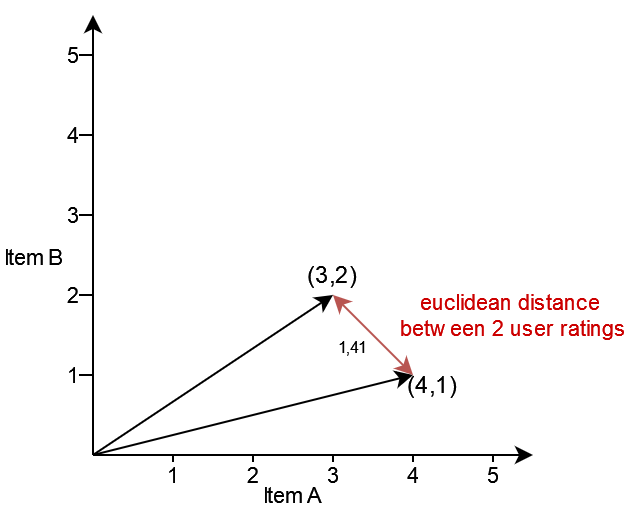
\includegraphics[width=\textwidth/2]{images/recommend/euclidian_distance_vis.drawio.png}
    \caption{\label{fig:recommend_euclid}Euclidean distance with two items and two user ratings}
    \end{figure}

    \item \textbf{Cosine distance}: This algorithm has a similar approach to the Euclidean distance, but with the cosine distance we compare the angle of the direction of the vectors \cite{miningOfMassiveDatasets}. In this case, we don't take into account the length of the vector, which can make the recommendation imprecise. This doesn't mean that the recommendation is worse than, for example, the Euclidean distance.

    \begin{figure}[h!]
    \centering
    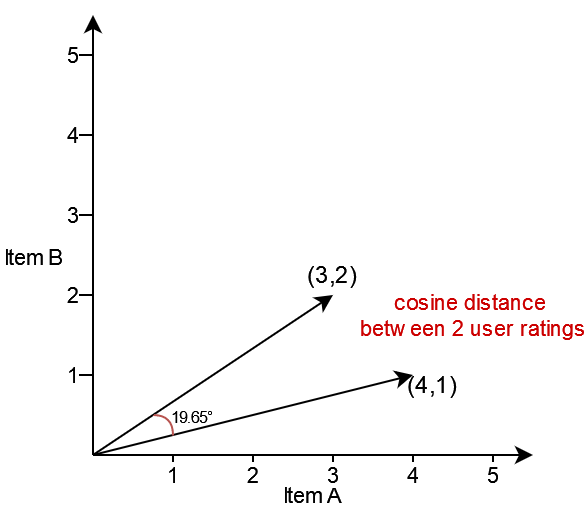
\includegraphics[width=\textwidth/2]{images/recommend/cosine_distance_vis.drawio.png}
    \caption{\label{fig:recommend_euclid}Cosine distance wit two items and two user ratings}
    \end{figure}

    \item \textbf{Pearson distance (Adjusted Cosine for Item based Collaborative Filtering)}: With Pearson, we use the same approach as with cosine distance, but with Pearson we normalise the ratings of all users before calculating a distance. Normalisation avoids the problem of favouring ratings from users with similar user biases to the target user \cite{miningOfMassiveDatasets}. A user bias occurs when a user rates items overwhelmingly positively or negatively. 

With the adjusted cosine (in item-based filtering domain), we don't want to normalise the item ratings because the item bias is the recommendation. Instead, we also normalise the user ratings as we do with the Pearson distance and then use the adjusted ratings for the cosine distance \cite{miningOfMassiveDatasets}.

\end{itemize}

Using these similarity measures, we can now select the most similar neighbours.

\subsection{Recommend an item}

Once we have found the k nearest neighbours, we can calculate an estimated rating of an unrated item for the target user. 

With user-based collaborative filtering, we look at the ratings of the k nearest users of an item that the target user hasn't rated. The average of these ratings can then be used as an indicator of whether or not the target user would like the item.

\begin{equation}
M_{u} = \frac{\sum_{i=1}^{k}{rating_i}}{k}
\label{mean}
\end{equation}

We can also take the weighted average to get a potentially more accurate recommendation:

\begin{equation}
M_{w} = \frac{\sum_{i=1}^{k}{rating_i * similarity_i}}{\sum_{i=1}^{k}{similarity_i}}
\label{weightedMean}
\end{equation}


This estimate reflects a possible rating of the target user. It also has the advantage that it can be used to test the recommendation system by trying to guess a rating that the user has already given and checking how much the estimated rating differs from the actual rating \cite{miningOfMassiveDatasets}. 

\section{Business Process Modelling Notations}

\label{sec:background_bpmn}

Business process modelling is an approach of describing the logical process in a business environment with a desired outcome \cite{bpm_review_framework}. Although many organisations use whiteboards or Microsoft Office to model processes, there is a trend towards using formal business process modelling notations (BPMN) \cite{ebpma-tec-standards, bpm_review_framework}. The benefits of formal BPMN are precision and reliability, so that everyone involved doesn't have to guess what different components of a notation mean \cite{ebpma-tec-standards}.

There are many BPMNs to choose from, \cite{bpm_review_framework} categorises them into different techniques:

\begin{itemize}
    
    \item \textbf{Flow Chart technique}: a simple, flexible and graphical approach to process modelling. Because of it's flexible design, it can also be used for logical sequences or as an organisation chart. 

    \begin{figure}[h]
    \centering
    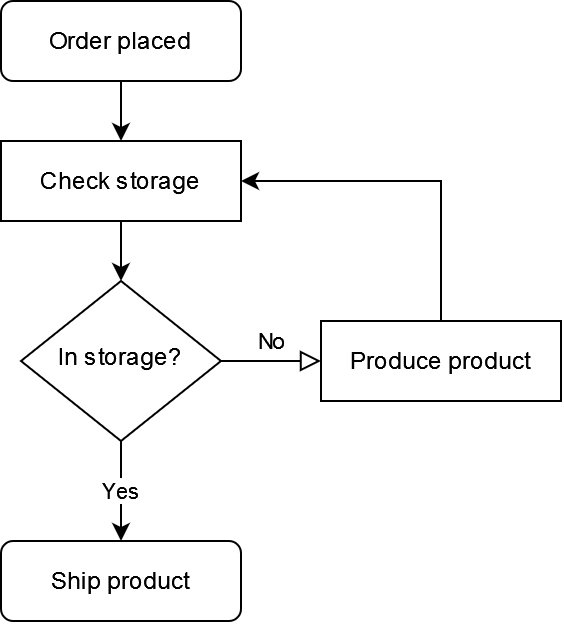
\includegraphics[width=\textwidth/3]{images/BPMN/flow_sample.drawio.png}
    \caption{\label{fig:bpmn_flow_chart}Flow Chart}
    \end{figure}

    
    \item \textbf{Data Flow diagrams}: a diagramming that visualises the flow of data or information between locations. It's often used between analysts and users because it's easy to understand and the connection points can be easily split to get more information.

    \begin{figure}[h]
    \centering
    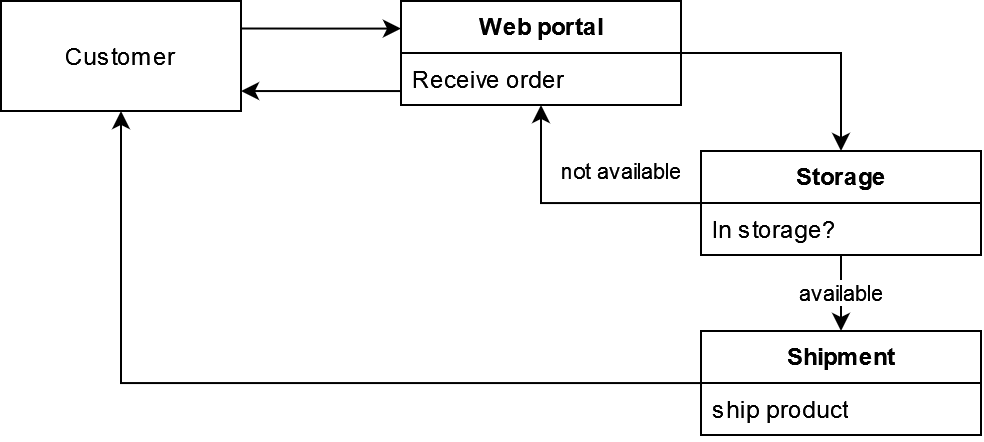
\includegraphics[width=\textwidth/3]{images/BPMN/dataflow_sample.drawio.png}
    \caption{\label{fig:bpmn_dataflow_diagram}Data Flow Diagram}
    \end{figure}

\newpage
    
    \item \textbf{Role activity diagrams}: a diagram that visualises a process from the perspective of a single role. Roles are abstract and describe a desired behaviour like an object in an object-oriented environment.
    
    \item \textbf{Role interaction diagrams}: A matrix-like diagram that describes a process through activities or connections between roles. Activities are actions a user can take, such as ordering a product. It's not as flexible as a flow chart, but still easy to understand.

    \begin{figure}[h]
    \centering
    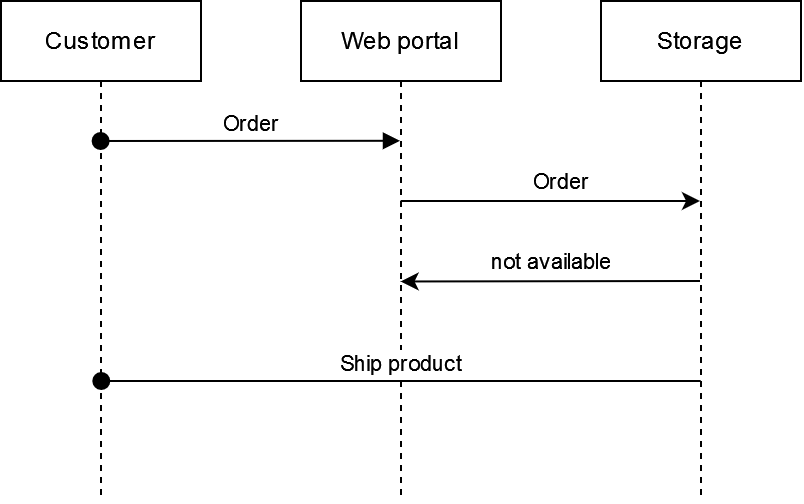
\includegraphics[width=\textwidth/2]{images/BPMN/role_int_sample.drawio.png}
    \caption{\label{fig:bpmn_RID_chart}Role interaction diagram}
    \end{figure}
    
    \item \textbf{Gantt Chart}: a matrix that describes a process through activities and time periods. The matrix can also includes names/actors or skill levels that perform an activity.

    \begin{figure}[h]
    \centering
    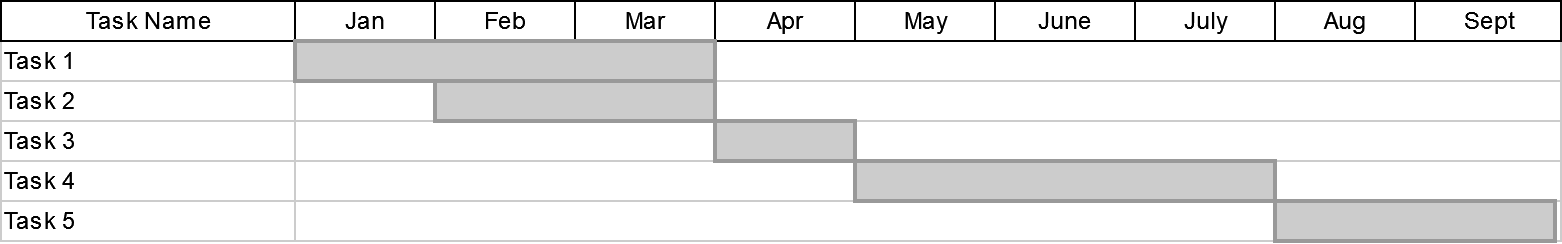
\includegraphics[width=\textwidth/2]{images/BPMN/Gnatt_sample.drawio.png}
    \caption{\label{fig:bpmn_gnatt_chart}Gantt Chart}
    \end{figure}
    
    \item \textbf{Integrated Definition for Function Modelling (IDEF)}: is a family of methods for modelling processes. The most useful are IDEF0 and IDEF3 for business process modelling and use activities that can also be represented as a sequence.

    \begin{figure}[h]
    \centering
    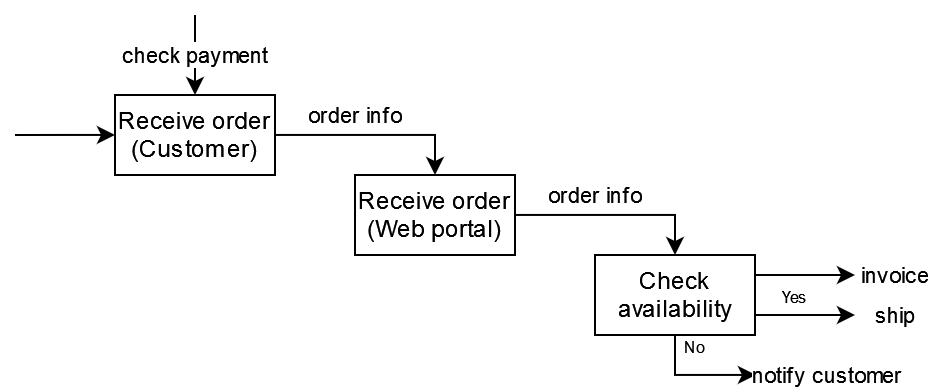
\includegraphics[width=\textwidth/2]{images/BPMN/idef_sample.drawio.png}
    \caption{\label{fig:bpmn_IDEF_diagram}IDEF0 diagram}
    \end{figure}
    
    \item \textbf{Coloured Petri-net}: is a graphical language that is useful when working with many processes that communicate and synchronise. The model contains modules, which in turn contain places and connections between them.
    
    \item \textbf{Object oriented methods}: combines data structures and behaviour. This allows an object to represent an entity that has a function in the real world and to interact with other entities.

    \begin{figure}[h]
    \centering
    
\includegraphics[width=\textwidth/2]{images/BPMN/uml_sample.drawio.png}
    \caption{\label{fig:bpmn_uml_diagram}UML diagram as a example of object oriented methods}
    \end{figure}
    
    \item \textbf{Workflow technique}: as the name suggests, data and information is passed from one node to another for further processing. Each node can take actions to achieve a common goal with other nodes. 
    
\end{itemize}

As we have seen, each technique has its advantages and its disadvantages.
\chapter{Requirements}

\chapter{Implementation}

\section{Kotlin Framework Ktor}

\section{Kotlin Library Ktorm}

\section{Recommender Implementation}
\chapter{Demonstration of the API}

\label{chap:demo}

To get a better understanding of the API and how it works, a demo application was developed. This demo application runs on the web, access the API and demonstrate the capabilities of the API.

\section{Conception}

\label{sec:demo_concept}

The demo application is written with the javascript framework Vue. To handle the requests to the recommendation API we use Axios.

\begin{figure}[h]
\centering
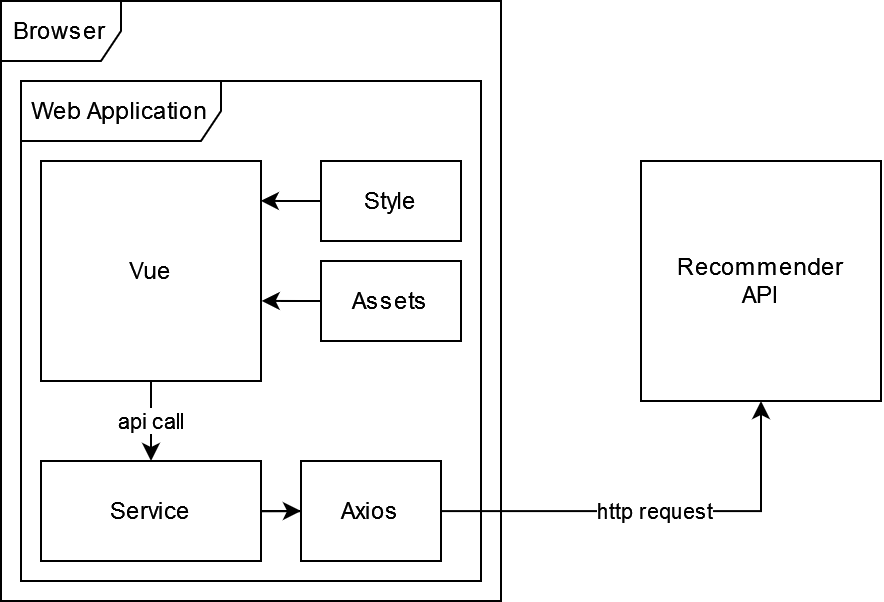
\includegraphics[width=\textwidth]{images/Demo_concept.drawio.png}
\caption{\label{fig:demo_concept}Concept of the Demo Application}
\end{figure}

\newpage

The service in overview \ref{fig:demo_concept} should be an interface or object that contains all possible requests to the API, and should convert the JSON data from the API into Javascript objects.

A UI is created to interact with the demo, the concept is shown in figure \ref{fig:ui_design_demo}.

\begin{figure}[h]
\centering
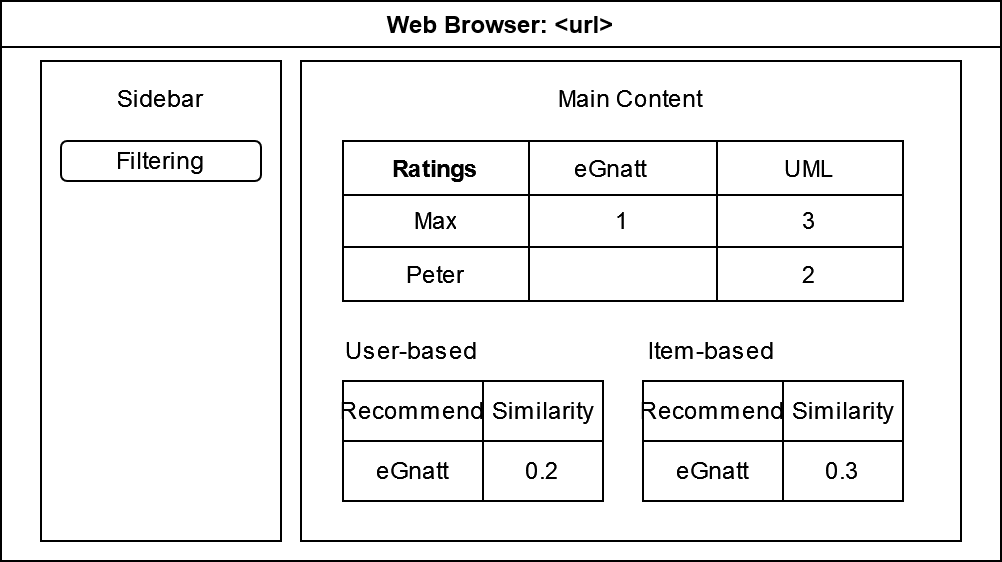
\includegraphics[width=\textwidth]{images/ui_concept.drawio.png}
\caption{\label{fig:ui_design_demo}Concept of the UI}
\end{figure}

\newpage

\section{Technologies}

\label{sec:demo_tec}

We now list the technologies we use in the demo application.

\subsection{Vite}

Vite is a development environment that builds and bundles Javascript, optimised for fast development. Vite addresses certain issues with component-based development and is the recommended build tool for Vue \cite{Vite}.

\subsection{Vue with Typescript}

Vue is a javascript framework that enables the usage of javascript, html and css in components \cite{Vue}. This makes code more reusable and also provides a level of security. Vue also provides plugins such as a router to display components on specific web routes \cite{VueRouter}. Typescript is a strongly typed language that is built on top of JavaScript and is developed and maintained by Microsoft and can also be used for Vue projects \cite{typescirpt}. 

\subsection{Axios}

Axios is an http client that can make xml http requests from the browser. We use Axios to make http requests to the API and convert JSON content to javascript objects.

\section{Implementation}

\label{sec:demo_impl}

Creating a Vue project creates some basic files: The main.ts, App.vue and the components directory. Within the index.ts, we define the Vue router and include styling files such as the base.css file.

\subsection{Router}

As mentioned above, the router is mounted on the application in main.ts and looks like this:

\newpage

\begin{minted}[frame=lines,framesep=2mm,baselinestretch=1.2,fontsize=\footnotesize,bgcolor=LightGray]{ts}
import { createApp } from 'vue'
import './assets/base.scss'
import App from "@/App.vue";
import HomeComponent from "@/components/struc/main/HomeComponent.vue";
import FilteringComponent from "@/components/struc/main/FilteringComponent.vue";
import {createRouter, createWebHashHistory} from "vue-router";
import UserComponent from "@/components/struc/main/UserComponent.vue";
import ItemComponent from "@/components/struc/main/ItemComponent.vue";
import AuthComponent from "@/components/struc/main/AuthComponent.vue";

const routes = [
    { path: '/', component: HomeComponent },
    { path: '/filtering', component: FilteringComponent },
    { path: '/user', component: UserComponent },
    { path: '/items', component: ItemComponent },
    { path: '/authentication', component: AuthComponent },
]

const router = createRouter({
    history: createWebHashHistory(),
    routes,
})

const app = createApp(App)
app.use(router)
app.mount('#app')
\end{minted}

The router allows easy switching between the defined components. Within the sidebar, switching to the routes can be done using buttons.

\subsection{Authentication}

To access the API, a token is required on each request. The demo application manages this by retrieving the token from the user with a text input, and then storing the token as a cookie so that the user is authenticated when they return. 

\begin{minted}[frame=lines,framesep=2mm,baselinestretch=1.2,fontsize=\footnotesize,bgcolor=LightGray]{html}
<script setup lang="ts">
import {ref} from "vue";
const inputToken = ref(localStorage.getItem('token') ?? '')
function save() {
  localStorage.setItem('token', inputToken.value)
}
</script>
<template>
  <div class="main-container">
    <div class="main-header anim" style="--delay: 0s">Authentication</div>
    <div class="input-auth-bar">
      <input v-model="inputToken" type="text" placeholder="Access Token">
      <a @click="save()" class="auth-check">Save</a>
    </div>
  </div>
</template>
\end{minted}

To make API requests with the token easier, a service.ts is defined that retrieves the token and appends it to each request.

\begin{minted}[frame=lines,framesep=2mm,baselinestretch=1.2,fontsize=\footnotesize,bgcolor=LightGray]{ts}
import axios from 'axios'

const API_URL = 'https://bpm.matthiasklenz.de'

const config = {
  baseURL: API_URL,
  timeout: 120000
}

export const service = axios.create(config)

service.interceptors.request.use(async (config) => {
  config.headers!.Authorization = `Bearer ${localStorage.getItem('token')}`
  return config
})

export default service
\end{minted}

\subsection{Filtering View}

The filtering view retrieves all ratings from all users and displays them in a table. To do this, all items are retrieved to show the names of the items.

\begin{minted}[frame=lines,framesep=2mm,baselinestretch=1.2,fontsize=\footnotesize,bgcolor=LightGray]{ts}
export type ItemSimilarity = {
  item: string
  similarity: number
}

export const getAllItems = () => service.get<ItemData[]>('/items')
\end{minted}

All users are retrieved to display the usernames within the table.

\begin{minted}[frame=lines,framesep=2mm,baselinestretch=1.2,fontsize=\footnotesize,bgcolor=LightGray]{ts}
export type UserData = {
  userid: number
  username: string
  info: string | null
}

export const getAllUsers = () => service.get<UserData[]>('/users')
\end{minted}

After the users have been retrieved, the user ratings are retrieved to display them in the table.

\begin{minted}[frame=lines,framesep=2mm,baselinestretch=1.2,fontsize=\footnotesize,bgcolor=LightGray]{ts}
export type UserRating = {
  userid: number
  ratings: Map<number, number>
}

export const getAllUserRatings = () 
    => service.get<UserRating[]>('/user/ratings')
\end{minted}

Once all the information has been retrieved, we can use Vue to create the table with the data provided.

\begin{minted}[frame=lines,framesep=2mm,baselinestretch=1.2,fontsize=\footnotesize,bgcolor=LightGray]{html}
<table>
  <thead>
  <tr>
    <th style="padding-right: 5rem">User</th>
    <th
        v-for="item in items"
        :key="item.id"
        v-on:click="setActiveItem(item.id)"
        v-bind:class="{ active: activeItem === item.id }"
        style="cursor: pointer"
    >
      {{ itemNameWithSimilarity(item.id) }}
    </th>
  </tr>
  </thead>
  <tbody>
    <tr
      v-for="user in userRatings"
      v-bind:class="{ active: activeUser === user.userid }"
      v-bind:key="user.userid"
    >
      <td v-on:click="setActiveUser(user.userid)" style="cursor: pointer">
        {{ usernameWithSimilarity(user.userid) }}
      </td>
      <td v-for="item in items" v-bind:key="item.id">
        {{ user.ratings[item.id.toString()] }}
     </td>
    </tr>
  </tbody>
</table>
\end{minted}

This completes the basic table. We now look at the similarities between users and items. To do this, the usernames and item names are clickable within the table. Clicking on a username will send the following request to the API

\begin{minted}[frame=lines,framesep=2mm,baselinestretch=1.2,fontsize=\footnotesize,bgcolor=LightGray]{ts}
export type UserSimilarity = {
  userid: number
  ratings: Map<number, number>
  similarity: number
}

export const getUserSimilarities = (
    user: number, 
    similarityMeasure: string = 'pearson'
) =>
  service.get<UserSimilarity[]>(
    `/userBased/similarities/${user}?SimilarityMeasure=${similarityMeasure}`
  )
\end{minted}

We can also include a similarity measure when trying to find the similarities between two users. The same can be done when making item similarity queries.

\begin{minted}[frame=lines,framesep=2mm,baselinestretch=1.2,fontsize=\footnotesize,bgcolor=LightGray]{ts}
export type ItemSimilarity = {
  item: string
  similarity: number
}

export const getItemSimilarities = (
    item: number, 
    similarityMeasure: string = 'pearson'
) =>
  service.get<ItemSimilarity[]>(
    `/itemBased/similarities/${item}?SimilarityMeasure=${similarityMeasure}`
  )
\end{minted}

When displaying user similarities, the user-based and item-based recommendations should also be displayed on-screen to show which item is recommended for the current user.


To get the user-based recommendations, we make the following request:

\newpage

\begin{minted}[frame=lines,framesep=2mm,baselinestretch=1.2,fontsize=\footnotesize,bgcolor=LightGray]{ts}
export type EstimatedRecommendations = {
  [key: string]: number
}

export const getUserRecommendations = (
  user: number,
  similarityMeasure: string = 'pearson',
  knn: number = 2,
  weighted: boolean = true
) =>
  service.get<EstimatedRecommendations>(
    `/userBased/recommendations/${user}?SimilarityMeasure=
    ${similarityMeasure}&knn=${knn}&weightedMean=${weighted}`
  )
\end{minted}

A different URL is used for the item-based recommendation:

\begin{minted}[frame=lines,framesep=2mm,baselinestretch=1.2,fontsize=\footnotesize,bgcolor=LightGray]{ts}
export const getItemRecommendations = (
  user: number,
  similarityMeasure: string = 'pearson',
  knn: number = 2,
  weighted: boolean = true
) =>
  service.get<EstimatedRecommendations>(
    `/itemBased/recommendations/${user}?SimilarityMeasure=
    ${similarityMeasure}&knn=${knn}&weightedMean=${weighted}`
  )
\end{minted}

\subsection{User View}

The User View lists all users and their information, users can be added, edited and deleted from the User View. User ratings can also be added in this view.

To add a user, a PUT request with the name and optional information is sent to the API.
\begin{minted}[frame=lines,framesep=2mm,baselinestretch=1.2,fontsize=\footnotesize,bgcolor=LightGray]{ts}
export const addUser = (username: string) 
    => service.put('/user', { username: username })
\end{minted}

To update user information, a UserData object is sent to the API, which then updates the information for the ID within the Data object.

\begin{minted}[frame=lines,framesep=2mm,baselinestretch=1.2,fontsize=\footnotesize,bgcolor=LightGray]{ts}
export const editUser = (userData: UserData) 
    => service.post('/user', userData)
\end{minted}

To delete a user, send a DELETE request with the userid.

\begin{minted}[frame=lines,framesep=2mm,baselinestretch=1.2,fontsize=\footnotesize,bgcolor=LightGray]{ts}
export const delUser = (id: number) => service.delete(`/user/${id}`)
\end{minted}

To add a rating, a POST request is sent with the itemId and userid along with the rating value.

\begin{minted}[frame=lines,framesep=2mm,baselinestretch=1.2,fontsize=\footnotesize,bgcolor=LightGray]{ts}
export const addRating = (userid: number, itemId: number, rating: number) =>
  service.post(
    '/user/rating', 
    { userid: userid, ratings: { [itemId]: rating } }
  )
\end{minted}

\subsection{Item View}

The Item view lists all items with their name and description. The table is structured so that the names and descriptions can be edited, deleted and submitted using a button. To edit an item, an ItemData object is sent and the API updates the entry based on the ID provided in the ItemData object.

\begin{minted}[frame=lines,framesep=2mm,baselinestretch=1.2,fontsize=\footnotesize,bgcolor=LightGray]{ts}
export const editItem = (data: ItemData) => service.post('/item', data)
\end{minted}

To delete an item, all the API needs is the ID.

\begin{minted}[frame=lines,framesep=2mm,baselinestretch=1.2,fontsize=\footnotesize,bgcolor=LightGray]{ts}
export const delItem = (id: number) => service.delete(`/item/${id}`)
\end{minted}

To add a new item, the ItemData is sent as a PUT request without the id.

\begin{minted}[frame=lines,framesep=2mm,baselinestretch=1.2,fontsize=\footnotesize,bgcolor=LightGray]{ts}
export const addItem = (name: string, description: string) =>
  service.put('/item', { name: name, description: description })
\end{minted}

\chapter{Deployment}

\label{chap:deployment}

This chapter describes how to set up and deploy the application in a production environment. We look at using Docker to host the application in a container for reproducible deployment, setting up MySQL as the database for the application, and using Github Actions for continuous integration and deployment as the application is developed further.

\section{Docker}

\label{sec:docker}

With Docker, we can run the application inside a container. A container is an isolated sandbox process on the host system that runs an image that provides a file system and other OS properties for the application to run. This allows a container to be moved, stopped, started, deleted or created \cite{docker}. The image is defined in the Docker file on the root of the project and can then be used with ease on your own host system. 

\begin{minted}[frame=lines,framesep=2mm,baselinestretch=1.2,fontsize=\footnotesize,bgcolor=LightGray]{docker}
FROM gradle:7.6.1-jdk17 as Builder

# Add backend sources
WORKDIR /src
RUN mkdir api
ADD . /src/api
ADD start.sh /src/api/run/start.sh

# Build jar
WORKDIR /src/api
RUN chmod u+x gradlew
RUN ./gradlew build --exclude-task test

# Prepare runtime
FROM openjdk:17-alpine

WORKDIR /run/
COPY --from=Builder /src/api/API/build/libs/*-all.jar /run/api.jar
COPY --from=Builder /src/api/run/start.sh /run/start.sh

EXPOSE 80

RUN chmod +x /run/start.sh

ENTRYPOINT ["/run/start.sh"]
\end{minted}

The docker image is also hosted on the official docker hub, so the docker command can automatically download the image from the docker hub. 

With docker compose, an extension of docker, we can more easily define volumes, prots or other metadata for the application inside a docker container. This compose file could look like:

\begin{minted}[frame=lines,framesep=2mm,baselinestretch=1.2,fontsize=\footnotesize,bgcolor=LightGray]{yaml}
version: '3.8'
services:
  recommender:
    image: 12build/bpmn_recommender:latest
    restart: always
    volumes:
      - ./config.yaml:/etc/configs/config.yaml
\end{minted}

\section{MySQL}

\label{sec:sql}

MySQL is an SQL (Structured Query Language) database developed by Oracle \cite{MySQL}. We use this database for no particular reason over any other SQL database. MySQL is a relational database and is used to store user data, item data and user ratings. MySQL can be set up similarly to the application using the official docker image.

\begin{minted}[frame=lines,framesep=2mm,baselinestretch=1.2,fontsize=\footnotesize,bgcolor=LightGray]{yaml}
version: '3.8'
services:
  recommender:
    image: 12build/bpmn_recommender:latest
    restart: always
    volumes:
      - ./config.yaml:/etc/configs/config.yaml
    depends_on:
      - database
  database:
    container_name: DB
    image: mysql:latest
    environment:
      MYSQL_ROOT_PASSWORD: ${MYSQL_ROOT_PASSWORD}
      MYSQL_DATABASE: api
      MYSQL_USER: api
      MYSQL_PASSWORD: ${MYSQL_API_PASSWORD}
    ports:
      - "3306:3306"
    volumes:
      - ./db_data:/var/lib/mysql
\end{minted}

Before starting the application for the first time, all tables have to be created within MySQL, this can be done as shown in Appendix \ref{code:sql_tables} and the tables can additionally be filled with dummy data.

\section{Github Actions}

\label{sec:github_actions}

The application is being developed on Github, using Github Actions for automated testing and deployment. Github Actions is a tool within Github to manage CI/CD or Continuous Integration and Deployment. We use it to build and test the application when pushing new code into the repository, and to deploy to the Docker Hub when a new release is created.

\begin{figure}[h!]
\centering
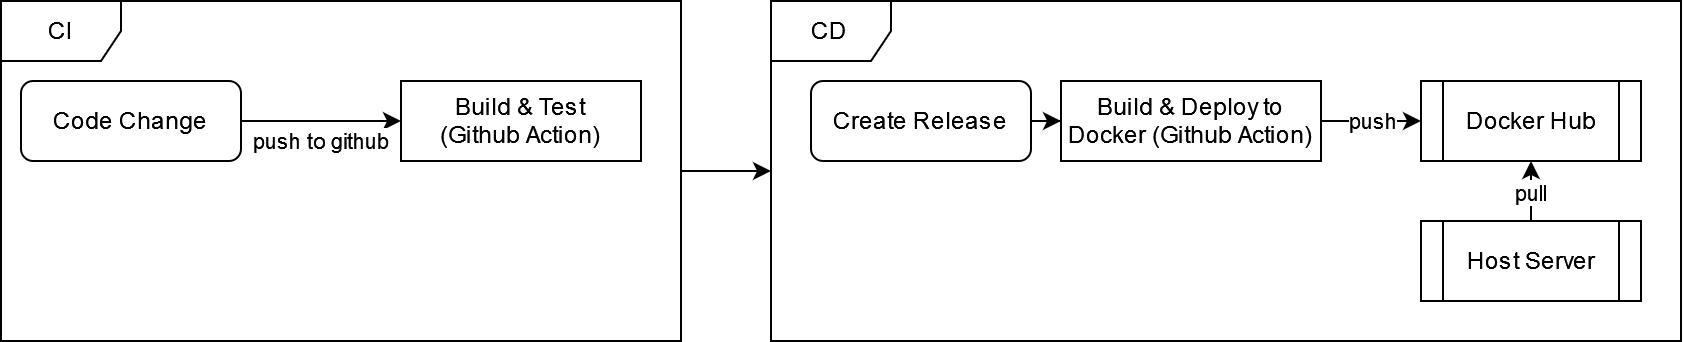
\includegraphics[width=\textwidth]{images/CICD_flow.drawio.png}
\caption{\label{fig:cicd}CI/CD Procedure}
\end{figure}


We define the build and test action shown in the Appendix \ref{code:github_build_and_test} and the deployment to the Docker Hub in the Appendix \ref{code:github_deploy}.
\chapter{Requirements Checking}

\label{chap:check_req}

In this chapter we check whether the functional and non-functional requirements defined in Chapter 4 have been met. An additional column is added to indicate whether the requirement has been met (+), partially met (0) or not met (-).

\section{Checking the Functional Requirements}

\label{seq:check_func_req}

\begin{longtable}{|p{1.2cm}||p{3.2cm}|p{8cm}|p{1cm}|}
    \hline
	  FR & Name & Description & +/0/-\\
	\hline
	FR 1 & Application & The application should be a REST Api written in Kotlin, accessible through the web & + \\
    \hline
	FR 2 & Authentication & Each Request to the API should be authenticated with a JSON web token & + \\
	\hline
    FR 3 & User Queries & The application should provide a route to any information about a user that the application has stored, such as the userid or username & + \\
	\hline
    FR 4 & User Mutation & The application should provide a Route to modify and add users & + \\
	\hline
    FR 5 & Item Queries & The application should provide a route for all information about an item that the application has stored & +\\
	\hline
    FR 6 & Item Mutations & The application should provide a Route to modify and add items & + \\
	\hline
    FR 7 & Rating Queries & The application should provide a route to get all the ratings of all users at once, or a specific user or item & +\\
	\hline
    FR 8 & User Similarity & The application should provide a route to get all similarities of a specific user with an http parameter to select a similarity algorithm and return a number  & +\\
	\hline
    FR 9 & Item Similarity & The application should provide a route to get all similarities of a specific item with an http parameter to select a similarity algorithm and return a number   & +\\
	\hline
    FR 10 & User-based Recommendation & The application should provide a way to get an estimated rating for any item a particular user hasn't rated, based on other users' ratings & + \\
	\hline
    FR 11 & Item-based Recommendation & The application should provide a way to get an estimated rating for any item that a particular user hasn't rated based on item ratings & + \\
	\hline
    FR 12 & Recommendation Algorithms & The application should provide the Euclidean, Cosine, Adjusted Cosine and Pearson algorithms for possible similarity measures. & + \\
	\hline
    FR 13 & Data Saving & The application should persistently store ratings, items and users in a MySQL database & + \\
	\hline
    FR 14 & Implementation Technologies & The application should be implemented with Kotlin and the Ktor server framework & + \\
	\hline
    FR 15 & Data refreshment & The estimated ratings and similarities should be updated on request or when a rating is added & + \\
	\hline
    FR 16 & Serialization of Input and Output & The application should serialise and deserialise data into JSON for communication between clients & +\\
	\hline

  \caption{Checking Functional Requirements}
  \label{tab:c-fas}
\end{longtable}

\section{Checking the Non-Functional Requirements}

\label{sec:check_non_func_req}

\begin{longtable}{|p{1.2cm}||p{3.2cm}|p{8cm}|p{1cm}|}
    \hline
	  FR & Name & Description & +/0/-\\
    \hline
    NFR 1 & Performance & The software shouldn't take more then 1gb of RAM and should minimize network traffic. & +\\
    \hline
    NFR 2 & Testing & The software should test all similarity and recommendation algorithms in a meaningful way, including unexpected input data. & +\\
    \hline
    NFR 3 & Usage & The API should be easy for a potential developer to use through intuitive routes, query parameters and API documentation. & +\\
    \hline
    NFR 4 & Extensions & The software should be extensible with more similarity measures. & +\\
    \hline
  \caption{Checking Non-functional Requirements}
  \label{tab:c-nfas}
\end{longtable}

\chapter{Conclusion}

\section{Limitations}

Das Kapitel muss eventuel wo anders hin da hier nochmal was neues kommt.

As in \cite{itemColFiltRecom} described, the recommendation algorithms used have problems with:

\begin{itemize}
    \item Sparsity: If the ratings table is nearly empty, the recommendation may break down, as single ratings can push the recommendation to an item that wouldn't normally be selected.
    \item Scalability: Currently, for each recommendation request, the API makes a database request for all ratings for all users and calculates the recommendation for a given user. This is currently acceptable as there aren't many items and reviews. This can be mitigated through caching but not solved... TODO
\end{itemize}

\appendix
% hier Anhänge einbinden
\chapter{Appendix}

\section{Application Entry Point}

\begin{minted}[frame=lines,framesep=2mm,baselinestretch=1.2,fontsize=\footnotesize,bgcolor=LightGray]{kotlin}
@Suppress("unused") // set in application.conf
fun Application.module() {
    val config = ConfigLoader().loadConfig().getOrElse {
        log.error(it.message)
        this.dispose()
        return
    }

    val logger = LoggerFactory.getLogger("api")

    val appModules = org.koin.dsl.module {
        single { config }
        single(qualifier("main")) { config.databases.main }
        single { logger }
        single { BpmDatabase() }
        single { JwtConfig(config.token) }
    }

    Server(this, appModules)
}
\end{minted}

\label{code:app_entry_point}

\section{Application Config}

\subsection{Ktor Application Config}

\begin{minted}[frame=lines,framesep=2mm,baselinestretch=1.2,fontsize=\footnotesize,bgcolor=LightGray]{kotlin}
ktor {
    deployment {
        port = 80
        port = ${?PORT}
    }
    application {
        modules = [ de.matthiasklenz.ApplicationKt.module ]
    }
}
\end{minted}
\label{code:ktor_app_conf}

\subsection{Loading the Config}

\begin{minted}[frame=lines,framesep=2mm,baselinestretch=1.2,fontsize=\footnotesize,bgcolor=LightGray]{kotlin}
class ConfigLoader {

    /**
     * Searches for the config:
     *
     * -> as a file in the run directory
     * -> as a file in a resource directory
     * -> as an Environment variable: "BPM_CONFIG"
     *
     * @return the Config of the API as a Result
     */
    fun loadConfig(): Result<Config> {
        val conf = loadConfigStr()
        return if (conf == null) {
            Result.failure(Error("Could not find Config!"))
        } else {
            Result.success(
                createYamlParser().decodeFromString(conf)
            )
        }
    }

    private fun loadConfigStr(): String? {
        return loadConfigFileFromResources()?.readText()
            ?: System.getenv("BPM_CONFIG")
            ?: null
    }

    private fun loadConfigFileFromResources(): File? {
        return if (File("config.yaml").exists()) {
            File("config.yaml")
        } else {
            File(
                Thread.currentThread().contextClassLoader!!.getResource(
                    "config.yaml"
                )?.path
                    ?: return null
            )
        }
    }

    private fun createYamlParser(): Yaml {
        val yamlConfig = Yaml.default.configuration.copy(
            polymorphismStyle = PolymorphismStyle.Property,
            polymorphismPropertyName = "type"
        )
        return Yaml(Yaml.default.serializersModule, yamlConfig)
    }
}

\end{minted}
\label{code:App_conf_loading}

\subsection{Config Object}

\begin{minted}[frame=lines,framesep=2mm,baselinestretch=1.2,fontsize=\footnotesize,bgcolor=LightGray]{kotlin}
@Serializable
data class Config(
    val token: String,
    val databases: Databases,
    val auth: Auth,
    val allowCORS: Boolean = false,
    val allowedCORS: List<String> = listOf()
)

@Serializable
data class Databases(
    val main: SqlDatabase,
)

@Serializable
data class SqlDatabase(
    val host: String,
    val port: Int,
    val schema: String,
    val user: String,
    val password: String,
)
\end{minted}
\label{code:App_conf_data}

\subsection{Config file}

\begin{minted}[frame=lines,framesep=2mm,baselinestretch=1.2,fontsize=\footnotesize,bgcolor=LightGray]{yaml}
token: W9je2oyqh6RGZdBfMJsVUR4
databases:
  main:
    host: localhost
    port: 3306
    schema: api
    user: api
    password: eN9LmPZKdnKEijFdjcuqHB2
allowCORS: false
allowedCORS: []
\end{minted}
\label{code:App_conf_yml}

\section{JWT authentication Configuration}

\begin{minted}[frame=lines,framesep=2mm,baselinestretch=1.2,fontsize=\footnotesize,bgcolor=LightGray]{kotlin}
class JwtConfig(jwtSecret: String) {
    companion object Constants {
        private const val CLAIM_USERINFO = "userinfo"
        private const val CLAIM_USER_ROLE = "userRole"
        private const val JWT_ISSUER = "de.matthiasklenz.upload"
        private const val JWT_REALM = "de.matthiasklenz.upload"
    }

    private val jwtAlgorithm = Algorithm.HMAC512(jwtSecret)
    private val jwtVerifier: JWTVerifier = JWT
        .require(jwtAlgorithm)
        .withIssuer(JWT_ISSUER)
        .build()

    /**
     * Generate a token for an authenticated user
     */
    fun generateToken(user: User): String = JWT.create()
        .withSubject("Authentication")
        .withIssuer(JWT_ISSUER)
        .withClaim(CLAIM_USERINFO, user.userinfo)
        .withClaim(CLAIM_USER_ROLE, user.role)
        .sign(jwtAlgorithm)

    /**
     * Configure the jwt ktor authentication feature
     */
    fun configureKtorFeature(
        config: JWTAuthenticationProvider.Config,
    ) = with(config) {
        verifier(jwtVerifier)
        realm = JWT_REALM
        validate {
            val userinfo = it.payload.getClaim(
                CLAIM_USERINFO
            ).asString()
            val userRole = it.payload.getClaim(
                CLAIM_USER_ROLE
            ).asString()

            if (userinfo != null && userRole != null) {
                User(userinfo, userRole)
            } else {
                null
            }
        }
    }

    /**
     * data object, that contains information of a user that is 
     * authenticated via jwt
     */
    data class User(
        val userinfo: String,
        val role: String,
    ) : Principal
}
\end{minted}
\label{code:JWT_conf}

\section{Routing}

\subsection{User}

\subsubsection{User Info}
\begin{minted}[frame=lines,framesep=2mm,baselinestretch=1.2,fontsize=\footnotesize,bgcolor=LightGray]{json}
{
  "userid": 8,
  "username": "Max",
  "info": "additional information"
}
\end{minted}
\label{code:user_info_json}

\subsubsection{User Ratings}
\begin{minted}[frame=lines,framesep=2mm,baselinestretch=1.2,fontsize=\footnotesize,bgcolor=LightGray]{json}
[
  {
    "userid": 1,
    "ratings": {
      "itemA": 2,
      "itemB": 1,
      "itemC": 5
    }
  },
  {
    "userid": 2,
    "ratings": {
      "itemA": 5,
      "itemB": 2
    }
  }
]
\end{minted}
\label{code:user_ratings_json}

\subsubsection{Create user data}
\begin{minted}[frame=lines,framesep=2mm,baselinestretch=1.2,fontsize=\footnotesize,bgcolor=LightGray]{json}
{
  "username": "Max",
  "information": "Admin"
}
\end{minted}
\label{code:user_create_json}

\subsubsection{Create user rating}
\begin{minted}[frame=lines,framesep=2mm,baselinestretch=1.2,fontsize=\footnotesize,bgcolor=LightGray]{json}
{
  "userid": 1,
  "ratings": {
    "itemA": 2,
    "itemB": 1,
    "itemC": 5
  }
}
\end{minted}
\label{code:user_reating_create_json}

\subsubsection{All User Info}
\begin{minted}[frame=lines,framesep=2mm,baselinestretch=1.2,fontsize=\footnotesize,bgcolor=LightGray]{json}
[
  {
    "userid": 1,
    "username": "Max",
    "info": "additional information"
  },
  {
    "userid": 2,
    "username": "Peter"
  }
]
\end{minted}
\label{code:user_infos_json}

\subsection{Item}

\subsubsection{Item info data}
\begin{minted}[frame=lines,framesep=2mm,baselinestretch=1.2,fontsize=\footnotesize,bgcolor=LightGray]{json}
{
  "id": 1,
  "name": "UML 2.0",
  "description": "..."
}
\end{minted}
\label{code:item_info_json}

\subsubsection{All item info data}
\begin{minted}[frame=lines,framesep=2mm,baselinestretch=1.2,fontsize=\footnotesize,bgcolor=LightGray]{json}
[
  {
    "id": 1,
    "name": "UML 2.0",
    "description": "..."
  },
  {
    "id": 2,
    "name": "Flow",
    "description": "..."
  }
]
\end{minted}
\label{code:items_info_json}

\subsubsection{Create item data}
\begin{minted}[frame=lines,framesep=2mm,baselinestretch=1.2,fontsize=\footnotesize,bgcolor=LightGray]{json}
{
  "name": "UML 2.0",
  "description": "..."
}
\end{minted}
\label{code:item_create_json}

\subsubsection{Modify item data}
\begin{minted}[frame=lines,framesep=2mm,baselinestretch=1.2,fontsize=\footnotesize,bgcolor=LightGray]{json}
{
  "id": 1,  
  "name": "UML 2.0",
  "description": "..."
}
\end{minted}
\label{code:item_modify_json}

\subsection{Recommend}

\begin{minted}[frame=lines,framesep=2mm,baselinestretch=1.2,fontsize=\footnotesize,bgcolor=LightGray]{json}
[
  {
    "userid": 2,
    "similarity": 0.23,
    "ratings": {
      "itemA": 2,
      "itemB": 1,
      "itemC": 5
    }
  },
  {
    "userid": 3,
    "similarity": 0.51,
    "ratings": {
      "itemA": 1,
      "itemB": 5,
      "itemC": 4
    }
  }
]
\end{minted}
\label{code:user_sim_json}

\section{Github Actions}

\subsection{Build and Test}
\begin{minted}[frame=lines,framesep=2mm,baselinestretch=1.2,fontsize=\footnotesize,bgcolor=LightGray]{yaml}
name: build
on:
  push:
    branches-ignore:
      - main
jobs:
  build:
    runs-on: ubuntu-latest
    steps:
      - name: Checkout code
        uses: actions/checkout@v2
      - name: Setup JDK 17
        uses: actions/setup-java@v2
        with:
          java-version: '17'
          distribution: 'adopt'
      - name: Build with Gradle
        env:
          GITHUB_TOKEN: ${{ secrets.GITHUB_TOKEN }}
          BPM_CONFIG: ${{ secrets.BPM_CONFIG }}
        run: ./gradlew --warning-mode all build
      - name: Run tests with Gradle
        env:
          GITHUB_TOKEN: ${{ secrets.GITHUB_TOKEN }}
          BPM_CONFIG: ${{ secrets.BPM_CONFIG }}
        run: ./gradlew --warning-mode all test
\end{minted}
\label{code:github_build_and_test}

\subsection{Deploy}

\begin{minted}[frame=lines,framesep=2mm,baselinestretch=1.2,fontsize=\footnotesize,bgcolor=LightGray]{yaml}
name: release
on:
  release:
    types: [ published ]
env:
  BPM_CONFIG: ${{ secrets.BPM_CONFIG }}
jobs:
  build-and-push-image:
    runs-on: ubuntu-latest
    steps:
      - name: Checkout
        uses: actions/checkout@v2
      - name: Login to Docker Hub
        uses: docker/login-action@v1
        with:
          username: ${{ secrets.DOCKERHUB_USERNAME }}
          password: ${{ secrets.DOCKERHUB_PASSWORD }}
      - name: Extract metadata (tags, labels) for Docker
        id: meta
        uses: docker/metadata-action@9ec57ed1fcdbf14dcef7dfbe97b2010124a938b7
        with:
          images: 12build/bpmn_recommender
      - name: Build Docker image
        uses: docker/build-push-action@v2
        with:
          context: .
          push: true
          tags: ${{ steps.meta.outputs.tags }}
          labels: ${{ steps.meta.outputs.labels }}
\end{minted}
\label{code:github_deploy}

\section{SQL}

\subsection{SQL tables}

\begin{minted}[frame=lines,framesep=2mm,baselinestretch=1.2,fontsize=\footnotesize,bgcolor=LightGray]{sql}
DROP TABLE bpm_user_recommendation;
DROP TABLE bpm_items;
DROP TABLE bpm_user;

CREATE TABLE bpm_items
(
    `id`          INT          NOT NULL AUTO_INCREMENT PRIMARY KEY,
    `name`        VARCHAR(255) NOT NULL,
    `description` TEXT         NOT NULL
);

CREATE TABLE bpm_user
(
    `id`   INT          NOT NULL AUTO_INCREMENT PRIMARY KEY,
    `name` VARCHAR(255) NOT NULL,
    `info` TEXT NULL DEFAULT NULL
);

CREATE TABLE bpm_user_recommendation
(
    `id`      INT NOT NULL AUTO_INCREMENT PRIMARY KEY,
    `userid`  INT NOT NULL,
    `item_id` INT NOT NULL,
    `rating`  INT NOT NULL DEFAULT 0,

    FOREIGN KEY (`userid`) REFERENCES bpm_user (id),
    FOREIGN KEY (`item_id`) REFERENCES bpm_items (id)
)
\end{minted}
\label{code:sql_tables}

\backmatter
\nocite{Knappen2009}
\nocite{Mittelbach2005}
\nocite{Schlosser2014}
\nocite{Sturm2012}
\nocite{Voss2010}

\printbibliography

\clearpage
\thispagestyle{empty}

Name: \fullname \hfill Matrikelnummer: \matnr \vspace{2cm}

\minisec{Erklärung}

Ich erkläre, dass ich die Arbeit selbständig verfasst und keine anderen als die angegebenen Quellen und Hilfsmittel verwendet habe.\vspace{2cm}

Ulm, den \dotfill

\hspace{10cm} {\footnotesize \fullname}
\end{document}
